\documentclass[10pt,a4paper]{article}
\usepackage[margin=2.2cm]{geometry}
\usepackage{fontspec}
\usepackage{kotex}
\setmainfont{Apple SD Gothic Neo}
\setsansfont{Apple SD Gothic Neo}
\usepackage{amsmath,amssymb}
\usepackage{graphicx}
\usepackage{booktabs}
\usepackage{caption}
\usepackage[dvipsnames]{xcolor}
\usepackage[colorlinks=true,linkcolor=MidnightBlue,citecolor=MidnightBlue,
            urlcolor=MidnightBlue]{hyperref}
\usepackage{titlesec}
\titleformat{\section}{\large\bfseries}{\thesection}{0.6em}{}
\titleformat{\subsection}{\normalsize\bfseries}{\thesubsection}{0.5em}{}
\captionsetup{font=small,labelfont=bf}
\setlength{\parskip}{0.35em}
\setlength{\parindent}{0pt}

\usepackage{mdframed}
\newmdenv[linewidth=0.4pt,linecolor=gray!60,backgroundcolor=gray!5,
          innertopmargin=6pt,innerbottommargin=6pt,skipabove=8pt,skipbelow=8pt]{claimbox}
\newcommand{\claim}[2]{\begin{claimbox}\textbf{주장.} #1\par\smallskip
  \textcolor{gray!70}{\textbf{반증 조건.} #2}\end{claimbox}}

\title{\bfseries 열쇠는 90일이었다\\[2pt]
\large 정의는 복원됐고, 헤드라인은 그래도 죽어 있다}
\author{월드모델 실험실 · 노트 $811$}
\date{2026-08-07}
\begin{document}\maketitle

\section{한 줄}

논문 $158$ 은 \emph{``우리가 닫은 문을 다시 열어 보니 열쇠가 없었다''}였다 ---
노트 $657$ 의 재는 코드가 사라졌고 자연스러운 정의 넷이 최고 $3/5$ 밖에 재현하지
못했다. 그때 \emph{``다섯째($90$일 창)는 새로 사전등록해야 쓴다''}로 문을 반쯤
남겨 뒀다. 이번에 그 사전등록을 했고 --- \textbf{열쇠가 맞았다.}

\begin{center}
\begin{tabular}{lccl}
\toprule
& E\_log$90$ & 노트 $657$ & 크기 배수 \\
\midrule
세계애니 & 단조 & 단조 \checkmark & $\mathbf{1.01 \cdot 1.02 \cdot 1.01}$ \\
모바일 & U & U \checkmark & $1.14 \cdot 0.99 \cdot 0.74$ \\
애니 & \textbf{U} & U \checkmark & $0.90 \cdot 0.86$ \\
웹툰 & 역U & 역U \checkmark & \\
\textcolor{BrickRed}{게임} & \textcolor{BrickRed}{\textbf{단조}} & U ✗ & $0.49 \cdot 0.87 \cdot 1.38$ \\
\bottomrule
\end{tabular}
\end{center}

\textbf{$4/5$ --- (좋) 발동. 노트 $656 \cdot 657$ 의 정의는 $90$일 log 기울기였다.}
세계애니의 배수 $1.01$ 셋은 같은 계산의 재현 수준이다. 애니는 $45$일 창에서
단조였다가 $90$일 창에서 U 로 돌아왔다 --- 창 길이가 무늬를 바꾸는 실물이다.

\begin{figure}[t]\centering
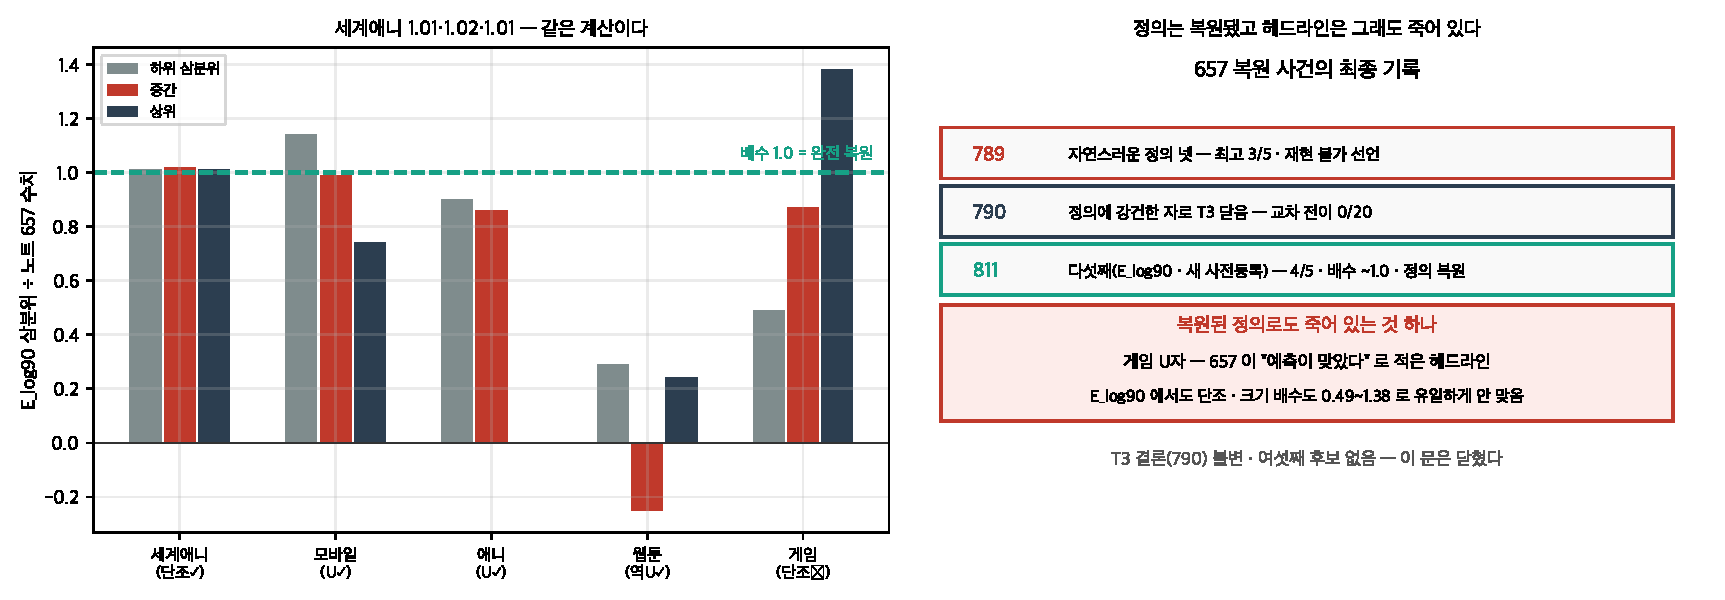
\includegraphics[width=0.92\textwidth]{figs/lock.pdf}
\caption{왼쪽: $657$ 수치 대비 배수 --- 세계애니가 $1.0$ 에 붙는다. 오른쪽: 세
걸음의 최종 기록과 남은 예외 하나.}
\end{figure}

\section{그래도 죽어 있는 것 하나}

\claim{\textbf{게임 U자 --- 노트 $657$ 이 ``예측이 맞았다''로 적은 헤드라인 ---
는 복원된 정의로도 단조다.} 크기 배수($0.49{\sim}1.38$)도 유일하게 안 맞는다.
행수 차($146$ 대 $149$ --- $90$일 조건이 셋을 떨어뜨림)가 후보이나 확정 불가.
\textbf{최종 기록: 정의는 복원됐고, 그 헤드라인 주장만 영구 재현 불가다.} 논문
$158$ 의 ``$657$ 이 이상하다고 본 게임이 실은 가장 센 도메인''(자기 전이 $+0.49$)
과 합치면 --- $657$ 의 게임 서사(U자 · 문제 있는 출시)는 무늬도 기제도 서지
않는다.}
{T$3$ 의 결론은 사전등록대로 \textbf{불변}이다 --- 노트 $790$ 은 정의 넷에 강건한
자(교차 전이 $0/20$)로 닫았고 E\_log$90$ 이 더해져도 ``안에서 세고 밖으로 안
간다''는 그대로다. \textbf{여섯째 후보는 없다 --- 이 문은 닫혔다.} T$3$ 의 남은
재개 조건은 (시간 $\times$ 대상) 궤적 원천 하나뿐이다.}

\section{규약 $41$ 의 값이 숫자로 남았다}

\claim{복원에 든 것: 사이클 셋($789 \cdot 790 \cdot 811$)과 정의 후보 다섯.
저장했더라면 든 것: $0$. \textbf{`lab/decay.py::E\_log90 · DEF\_RECOVERED} 로
이번 복원 자체를 저장소에 뒀고 감사표가 지킨다 --- 이 각주가 다시 고아가 되면
감사가 잡는다. 주 갈래 예측 $5$연속 적중.}
{크기 배수 예측(게임 $\pm 30\%$)은 틀렸다 --- 게임은 크기까지 안 맞는 유일한
도메인이고, 그것이 무늬 불일치와 정합한다는 점에서 \textbf{틀림이 이야기를
강화한 드문 경우}다.}

\end{document}
